\chapter{Plotting with PyPlot}
\label{ch:pyplot}

%%%%%%%%%%%%%%%%%%%%%%%%%%%%%%%%%%%%%%%%  intro
\section{matplotlib.pyplot}\label{s:pyplot_intro}
Matplotlib and its PyPlot environment is a versatile Python plotting
library which produces publication quality figures in a variety of
hard-copy formats such as EPS, PDF, and PNG.  With PyPlot you can
generate scatter and line plots, histograms, power spectra, bar
charts, error-charts, pie charts, and many more with just a few lines
of code. For the power user, you have full control of line styles,
font properties, axes properties, and so on. For useful examples of 
astronomy plots that can be generated with PyPlot, see Leonardo 
Ubeda's astroplotlib library at \href{http://astroplotlib.stsci.edu/}
{http://astroplotlib.stsci.edu/}


%%%%%%%%%%%%%%%%%%%%%%%%%%%%%%%%%%%%%%%%  Create simple scatter plot
\section{Create a Simple Scatter Plot}\label{s:simple_plot}

We'll start by making a simple scatter plot, demonstrating some of 
the PyPlot options, and saving our plot in a PDF format. 

First, we need to read in some data, as we learned in Chapter~\ref{ch:fits},
using the two files `flux\_vs\_time\_A.dat' and `flux\_vs\_time\_C.dat' found
in /user/gunning/Python\_Training/.

\begin{alltt}
\pytab from astropy.io import ascii
\pytab data_A = ascii.read('flux_vs_time_A.dat', names=['Time',  \textbackslash 
\ldots 'Flux_diff', 'Flux_err', 'Flux_linear_fit'])
\pytab data_C = ascii.read('flux_vs_time_C.dat', names=['Time',  \textbackslash 
\ldots 'Flux_diff', 'Flux_err', 'Flux_linear_fit'])
\end{alltt}

The time is in Modified Julian Date (MJD) and the remaining 
columns are flux percent differences and are dimensionless. 
%(The fluxes are of a standard white dwarf for a WFC3 monitoring 
%program. The two datasets are from different amplifiers
%on the WFC3 two-chip mosaic.)

Now we will import PyPlot and make our first plot, 
using a \textit{figure} object...

\begin{alltt}
\pytab import matplotlib.pyplot as pyplot
\pytab figure, ax = pyplot.subplots()
\end{alltt}

Now we can begin to plot into the \textit{figure} object, via the \textit{ax} 
axis created in the previous step. Each subsequent call to the inherited 
\textit{ax.plot} method will update the overall plot. The next two calls
plot the two sets of flux differences as scatter plots in blue and red,
respectively.

\begin{alltt}
\pytab ax.scatter(data_A['Time'], data_A['Flux_diff'], c='blue')
\pytab ax.scatter(data_C['Time'], data_C['Flux_diff'], c='red')
\pytab figure.show()
\end{alltt}

The \textit{figure.show()} command displays our changes onto the \textit{figure}
object.

We should add axis labels...

\begin{alltt}
\pytab ax.set_xlabel('Time [MJD]', fontsize=20)
\pytab ax.set_ylabel('Flux Diff [%]',  fontsize=20)
\pytab figure.show()
\end{alltt}

Finally let's save the figure. We can save as a PDF, PNG, TIFF, and
other file types; we need only to type the appropriate extension.

\begin{alltt}
\pytab figure.savefig('flux_vs_time_1.pdf')
\end{alltt}


%%%%%%%%%%%%%%%%
\begin{figure}[tbp]
  \centering
    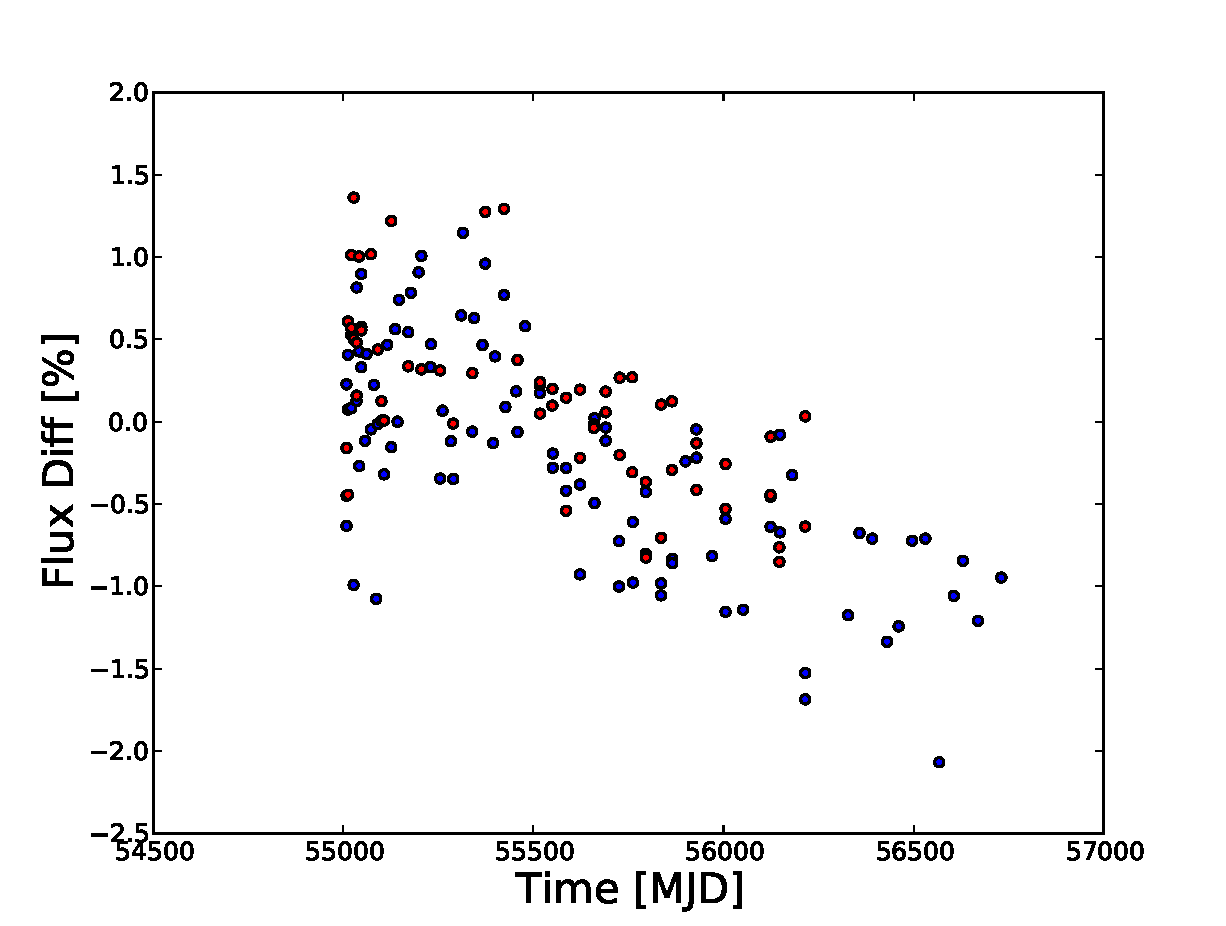
\includegraphics[scale=0.55]{flux_vs_time_1.pdf}
    \caption{Our first plot.}
  \label{fig:flux_vs_time_1}
\end{figure}
%%%%%%%%%%%%%%%%

%%%%%%%%%%%%%%%%%%%%%%%%%%%%%%%%%%%%%%%%  Markers, lines, and legends
\section{Markers, Lines, and Legends}\label{s:markers_lines_legends}  %Plot customizations

We have a plot! But we are not yet finished.
PyPlot has many, many options available for you to customize
your plot. We'll demonstrate just a few for markers, lines, and legends. 

We can play with the marker type (\textit{marker}), size (\textit{s}), and 
transparency (\textit{alpha}) of our of scatter plots' points. We first
need to clear the  \textit{axis} object with the \textit{ax.clear()} command.

\begin{alltt}
\pytab ax.clear()
\pytab ax.scatter(data_A['Time'], data_A['Flux_diff'], \textbackslash 
\ldots   c='blue', marker='x', s=30, alpha=0.75)
\pytab ax.scatter(data_C['Time'], data_C['Flux_diff'], \textbackslash 
\ldots   c='red', marker='d', s=30, alpha=0.75)
\pytab ax.set_xlabel('Time [MJD]', fontsize=20)
\pytab ax.set_ylabel('Flux Diff [%]', fontsize=20)
\pytab figure.show()
\end{alltt}

The plot would be cleaner if we added a legend.

\begin{alltt}
\pytab ax.clear()
\pytab ax.scatter(data_A['Time'], data_A['Flux_diff'], \textbackslash 
\ldots   c='blue', marker='x', s=25, alpha=0.75, label='Amp A')
\pytab ax.scatter(data_C['Time'], data_C['Flux_diff'], \textbackslash 
\ldots   c='red', marker='d', s=25, alpha=0.75, label='Amp C')
\pytab ax.set_xlabel('Time [MJD]', fontsize=20)
\pytab ax.set_ylabel('Flux Diff [%]', fontsize=20)
\pytab ax.legend(loc='best', scatterpoints=1)
\pytab figure.show()
\end{alltt}

The \textit{ax.legend(loc='best')} command will try to find the least busy section 
of your plot and stick the legend there. 

Next let's plot lines with the linear fits from our data:

\begin{alltt}
\pytab ax.plot(data_A['Time'], data_A['Flux_linear_fit'], \textbackslash 
\ldots  c='blue', ls='-.', linewidth=2, label='Amp A Fit')
\pytab ax.plot(data_C['Time'], data_C['Flux_linear_fit'], \textbackslash 
\ldots  c='red', ls=':', linewidth=2, label='Amp C Fit')
\pytab ax.legend(loc='best', scatterpoints=1)
\pytab figure.show()
\end{alltt}

Notice the \textit{ls} option is how we select our line type. 
Suppose we want to denote the 0.0 flux difference with a dashed line and the
MJD date 56250.0 with a green line:

\begin{alltt}
\pytab ax.axhline(0.0, color='k', ls='--', linewidth=1)  
\pytab ax.axvline(56250.0, color='green', ls='-', linewidth=2) 
\pytab figure.show()
\end{alltt}

%%%%%%%%%%%%%%%%
\begin{figure}[tbp]
  \centering
    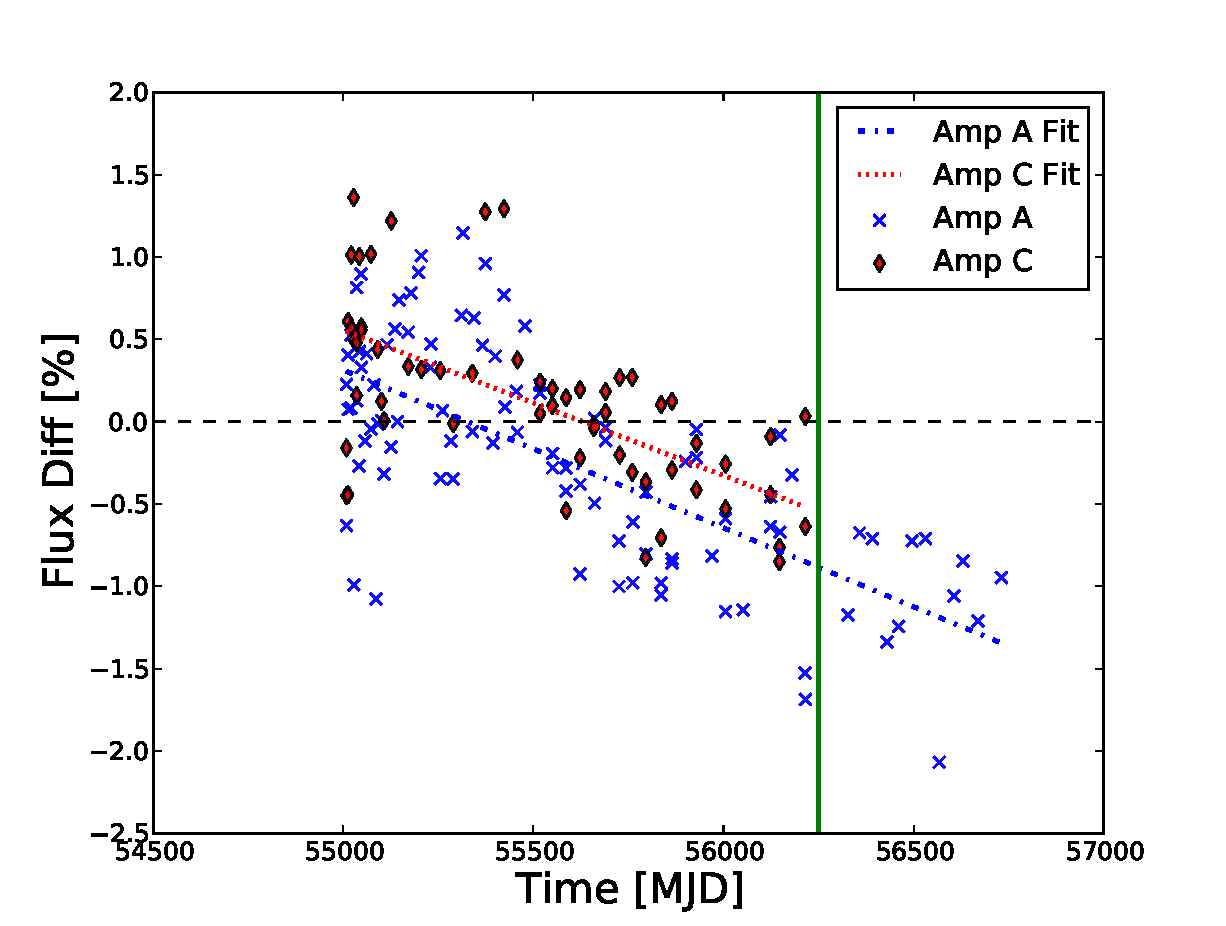
\includegraphics[scale=0.55]{flux_vs_time_2.pdf}
    \caption{Our customized plot.}
  \label{fig:flux_vs_time_2}
\end{figure}
%%%%%%%%%%%%%%%%

We now have a personalized plot! (It doesn't have to be pretty.) Let's save it.

\begin{alltt}
\pytab figure.savefig('flux_vs_time_2.pdf')
\end{alltt}

Other options can be found on the Matplotlib PyPlot site listed in Chapter~\ref{ch:links}. 

For different color names, see \href{http://www.w3schools.com/html/html_colornames.asp}
{http://www.w3schools.com/html/html\_colornames.asp}

{\color{blue} {\sf\small EXERCISES}} \\
{\it Exercise \arabic{exercise} \stepcounter{exercise}:  \\
Play with different colors, markers, lines, etc.}


%http://matplotlib.org/1.2.1/examples/pylab_examples/show_colormaps.html

%%%%%%%%%%%%%%%%%%%%%%%%%%%%%%%%%%%%%%%%  Error bars
\section{Error Bars}\label{s:error_bars}

We have columns giving our error in flux percent difference. We can display them on our plot as
error bars using the \textit{errorbar} function:

\begin{alltt}
\pytab ax.clear()
\pytab ax.scatter(data_A['Time'], data_A['Flux_diff'], \textbackslash
\ldots c='blue', s=10)
\pytab ax.errorbar(data_A['Time'], data_A['Flux_diff'], \textbackslash 
\ldots yerr=data_A['Flux_err'], c='k', marker=None, ls='None')
\pytab figure.show()
\end{alltt}

%%%%%%%%%%%%%%%%%%%%%%%%%%%%%%%%%%%%%%%%  Display year-month-day
\section{Display Year-Month-Day Dates as Tick Labels}\label{s:dates}

MJD is a convenient format for plotting time. But who 
thinks in MJD? Let's convert MJD to year-month-day and display them 
on the x-axis. In Python this is a little tricky. We will show one way to do
it; you may be able to find a better way.

Let's continue working on the plot we began in the Error Bars section.
We first need to import \textit{Time} from \textit{astropy}, and then save
into a list the MJD dates that are currently displayed as tick labels (converting them into
floats as we do so).

\begin{alltt}
\pytab from astropy.time import Time
\pytab time\_MJD = [float(item.get\_text()) \textbackslash
\ldots for item in ax.get\_xticklabels()]
\end{alltt}

We next need to convert the MJD date list into a \textit{Time} object. 

\begin{alltt}
\pytab time\_convert = Time(time\_MJD, format='mjd', scale='utc')
\end{alltt}

Now we can convert the MJD dates into year-month-day dates. Because
the conversion also includes minutes and seconds, which we do not want
in this example, we will use the \textit{split()} method to extract just the 
year-month-days and append them into a new list. 

\begin{alltt}
\pytab time\_ymd\_long = time\_convert.iso
\pytab time\_ymd\_short = []
\pytab for date in time\_ymd\_long:
\ldots    time\_ymd\_short.append(date.split(' ')[0])
\end{alltt}

Finally we can display our new tick labels on the x-axis and save the figure.

\begin{alltt}
\pytab ax.set\_xticklabels(time\_ymd\_short)
\pytab ax.set\_xlabel('Time', fontsize=20)
\pytab ax.set\_ylabel('Flux Diff [%]', fontsize=20)
\pytab figure.show()
\pytab figure.savefig('flux_vs_time_3.pdf')
\end{alltt}

See \href{http://astropy.readthedocs.org/en/latest/time/}{http://astropy.readthedocs.org/en/latest/time/} for more examples.

%%%%%%%%%%%%%%%%
\begin{figure}[tbp]
  \centering
    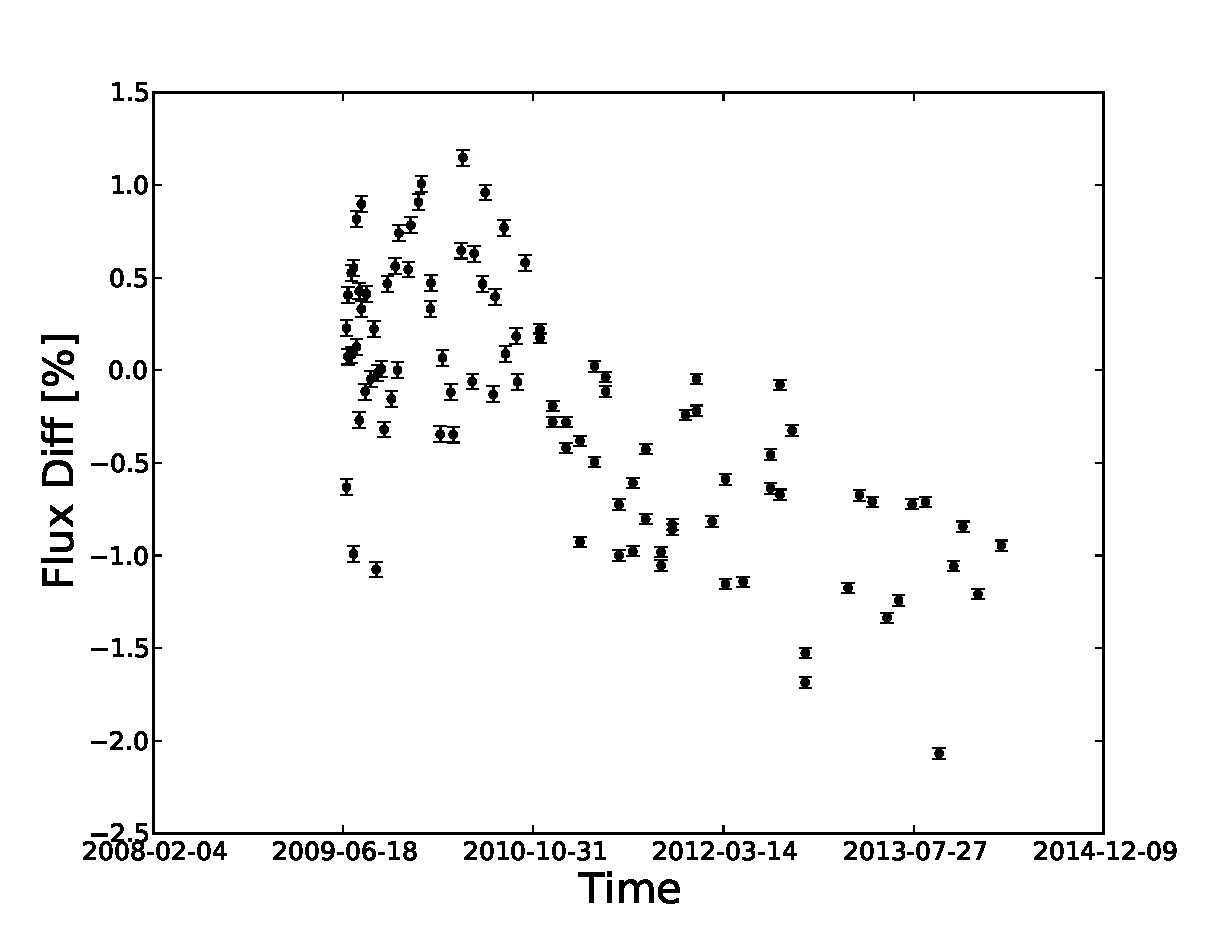
\includegraphics[scale=0.55]{flux_vs_time_3.pdf}
    \caption{Our error bar plot with x-axis tick labels converted from MJD to year-month-day.}
  \label{fig:flux_vs_time_3}
\end{figure}
%%%%%%%%%%%%%%%%

{\color{blue} {\sf\small EXERCISES}} \\
{\it Exercise \arabic{exercise} \stepcounter{exercise}:  \\
Assume you do not have the MJD list. Starting from the list of year-month-day, convert your axis to days from the start date
and display the tick labels. 
So your first tick label should be 0, and your x-axis title should be something like `Days since 2008-02-04'.}


%\section{Fitting Routines}

%We do not recommend using Python's fitting routines, as they have been 
%known to have issues. In general, you will want to write your own or use
%tried-and-true routines from IRAF/PyRAF.  (For instance, the linear fit lines 
%we plotted earlier were calculated with IRAF's TLINEAR task.)


%%%%%%%%%%%%%%%%%%%%%%%%%%%%%%%%%%%%%%%%  Display plots side-by-side
\section{Display Plots Side-by-Side}\label{s:mulitplots}

As with most plotting matters in Python, there's more than one way to 
display multiple plots on the same figure. We will demonstrate making
a simple 2$\times$1 multiple plot with just the \textit{subplot()} method. 

Let's make a new figure, resizing it to 10$\times$10 inches so we can better see our plots.
Then we'll place the first plot at position 211. The first number (2) denotes 
how many plots are to be placed vertically; the second number (1) denotes
how many plots are to be placed horizontally; and the third number (1) denotes
where the current plot is to be placed in this grid (in this case, the first position). 
If, say, we wanted a 2$\times$2 grid and wanted to place a plot in the lower right corner,
we would write 224.


\begin{alltt}
\pytab figure = pyplot.figure(figsize = (10,10))
\pytab ax1 = pyplot.subplot(211, title='Amp A')
\pytab ax1.scatter(data_A['Time'], data_A['Flux_diff'], c='blue')
\end{alltt}

We can make the top plot's x-axis invisible... 

\begin{alltt}
\pytab pyplot.setp(ax1.get_xticklabels(), visible=False)
\end{alltt}

We next place the second plot at position 212. We use the \textit{sharex} and \textit{sharey} options
to force the second plot's  axes to match the first's.

\begin{alltt}
\pytab ax2 = pyplot.subplot(212, title='Amp C', sharex=ax1, sharey=ax1)
\pytab ax2.scatter(data_C['Time'], data_C['Flux_diff'], c='red')
\end{alltt}

We'll finish by setting the x and y axes labels and saving the figure.

\begin{alltt}
\pytab ax1.set_ylabel('Flux Diff [%]', fontsize=15)
\pytab ax2.set_ylabel('Flux Diff [%]', fontsize=15)
\pytab ax2.set_xlabel('Time [MJD]', fontsize=15)
\pytab figure.show()
\pytab figure.savefig('flux_vs_time_4.pdf')
\end{alltt}

%%%%%%%%%%%%%%%%
\begin{figure}[tbp]
  \centering
    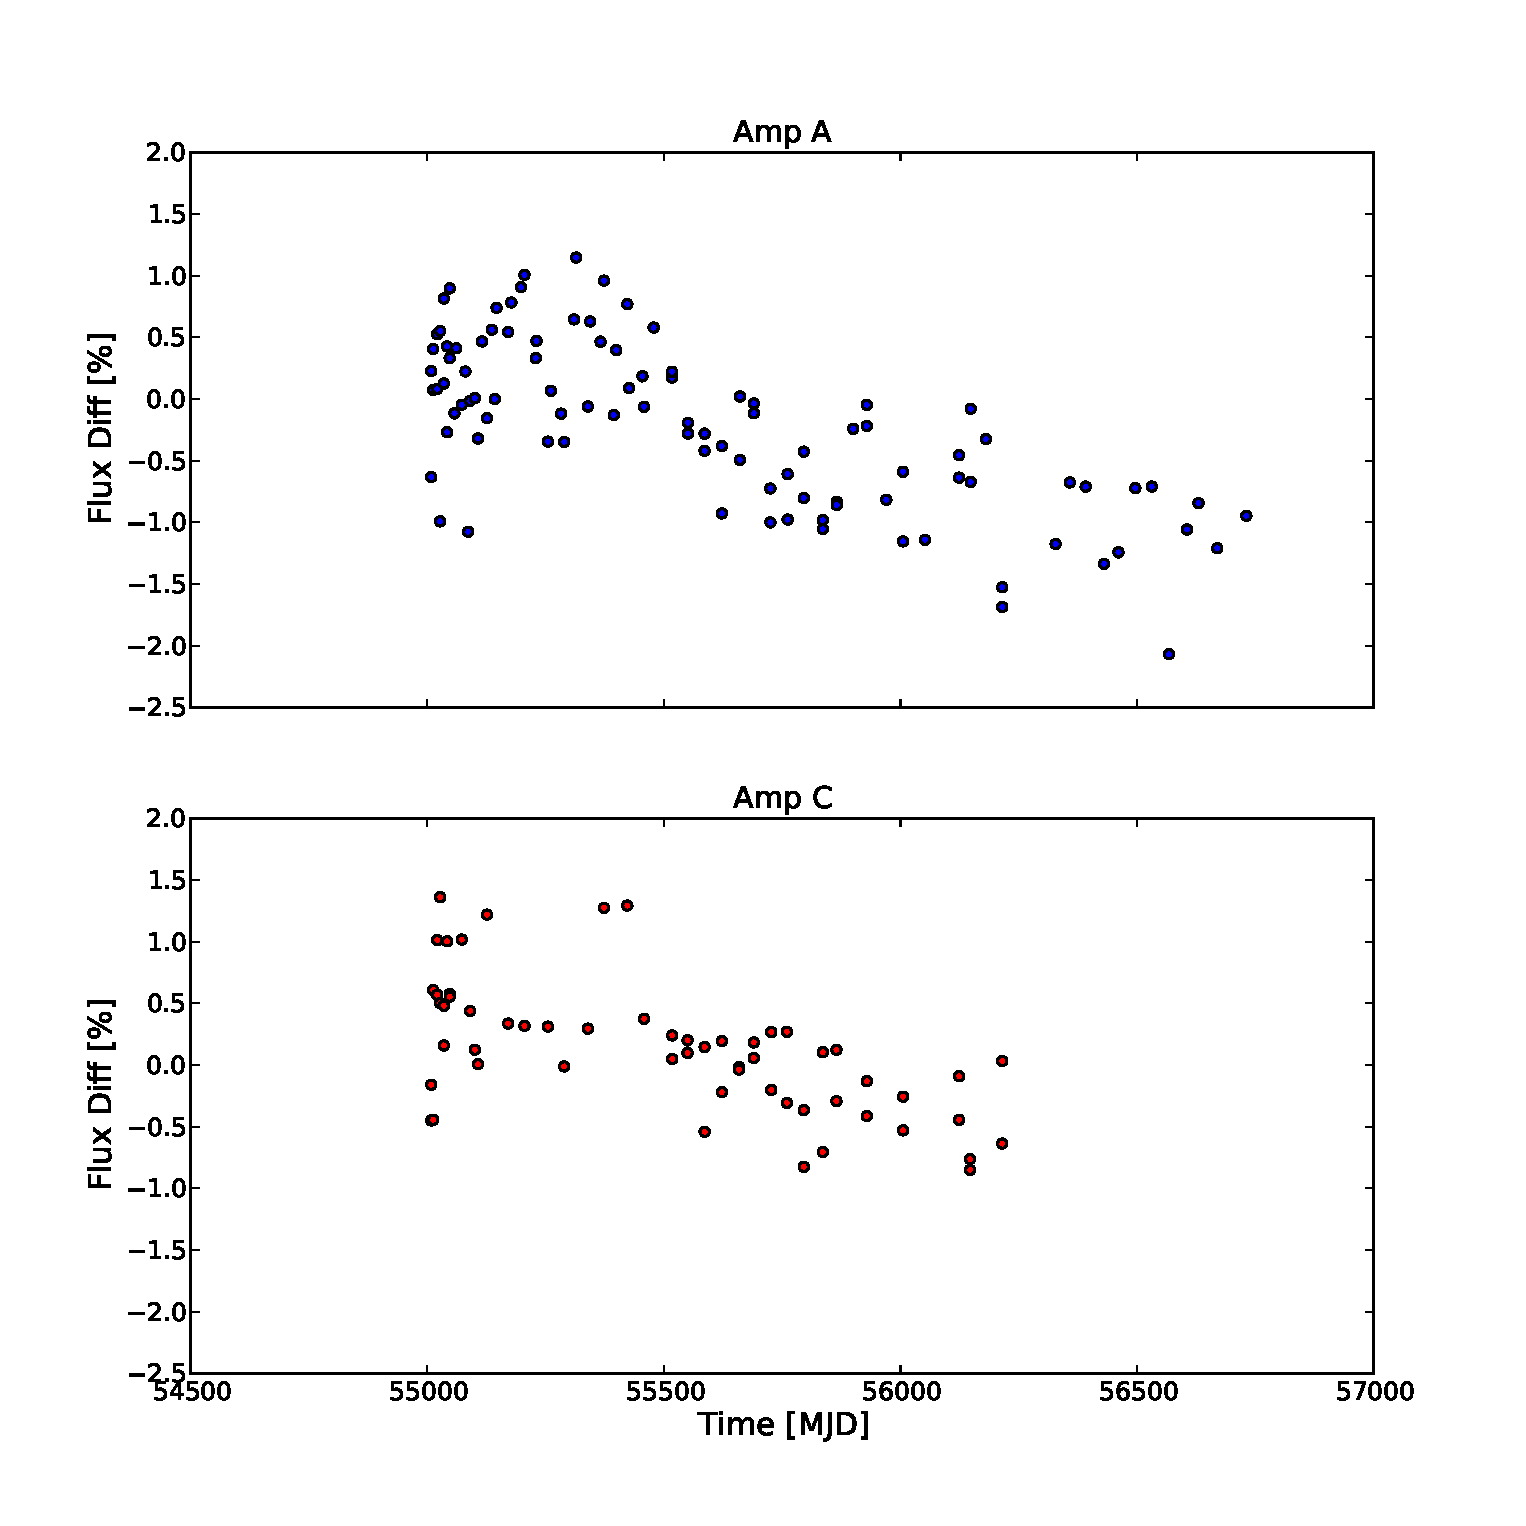
\includegraphics[scale=0.35]{flux_vs_time_4.pdf}
    \caption{Our 2$\times$1 multiple plot.}
  \label{fig:flux_vs_time_4}
\end{figure}
%%%%%%%%%%%%%%%%

{\color{blue} {\sf\small EXERCISES}} \\
{\it Exercise \arabic{exercise} \stepcounter{exercise}:  \\
Create a 2$\times$2 grid and display the above two plots in the upper two areas. Then display our first plot
 from Section \ref{s:simple_plot} below them, filling the entire lower area.}


%%%%%%%%%%%%%%%%%%%%%%%%%%%%%%%%%%%%%%%%  Display a FITS image
\section{Display a FITS Image}\label{s:display_fits}

Copy the FITS file `ibsa01fpq\_flt.fits' from /user/gunning/Python\_Training/ to your current working directory. It
is a WFC3/IR image of a corner of the galaxy M51.
% Note that the image is non-proprietary. From Prop ID 12490, Visit 01. 

We will use astropy's \textit{fits} package to open the file, as we learned in Chapter~\ref{ch:fits},
and extract the image data from the SCI extension.  

\begin{alltt}
\pytab import astropy.io.fits as fits
\pytab image = fits.open('ibsa01fpq_flt.fits')
\pytab sci_data = image['sci'].data
\pytab pylplot.clf()
\pytab pyplot.gray()
\pytab pyplot.imshow(sci_data, vmin=0, vmax=60)
\pytab pyplot.show()
\pytab image.close()
\end{alltt}

{\color{blue} {\sf\small EXERCISES}} \\
{\it Exercise \arabic{exercise} \stepcounter{exercise}:  \\
How does that look? Mess with the \textit{vmin} and \textit{vmax} to see if you can improve the scaling.
The \textit{pyplot.gray()} command sets the plot to greyscale. Take a look at the plot without it.}

We can add labels:  

\begin{alltt}
\pytab pyplot.title('M51', fontsize=20)
\pytab pyplot.xlabel('x pixels', fontsize=15)
\pytab pyplot.ylabel('y pixels', fontsize=15)
\end{alltt}

Before saving, we can try annotating features in our image. In this example,
we point to a star near pixel coordinates (640, 810) with an arrow.

\begin{alltt}
\pytab pyplot.annotate('star', xy=(640,810),  xytext=(520,770), \textbackslash
\ldots color='white', arrowprops=dict(facecolor='white', width=3.5))
\pytab pyplot.savefig('M51.pdf')
\end{alltt}

%%%%%%%%%%%%%%%%
\begin{figure}[H]
  \centering
    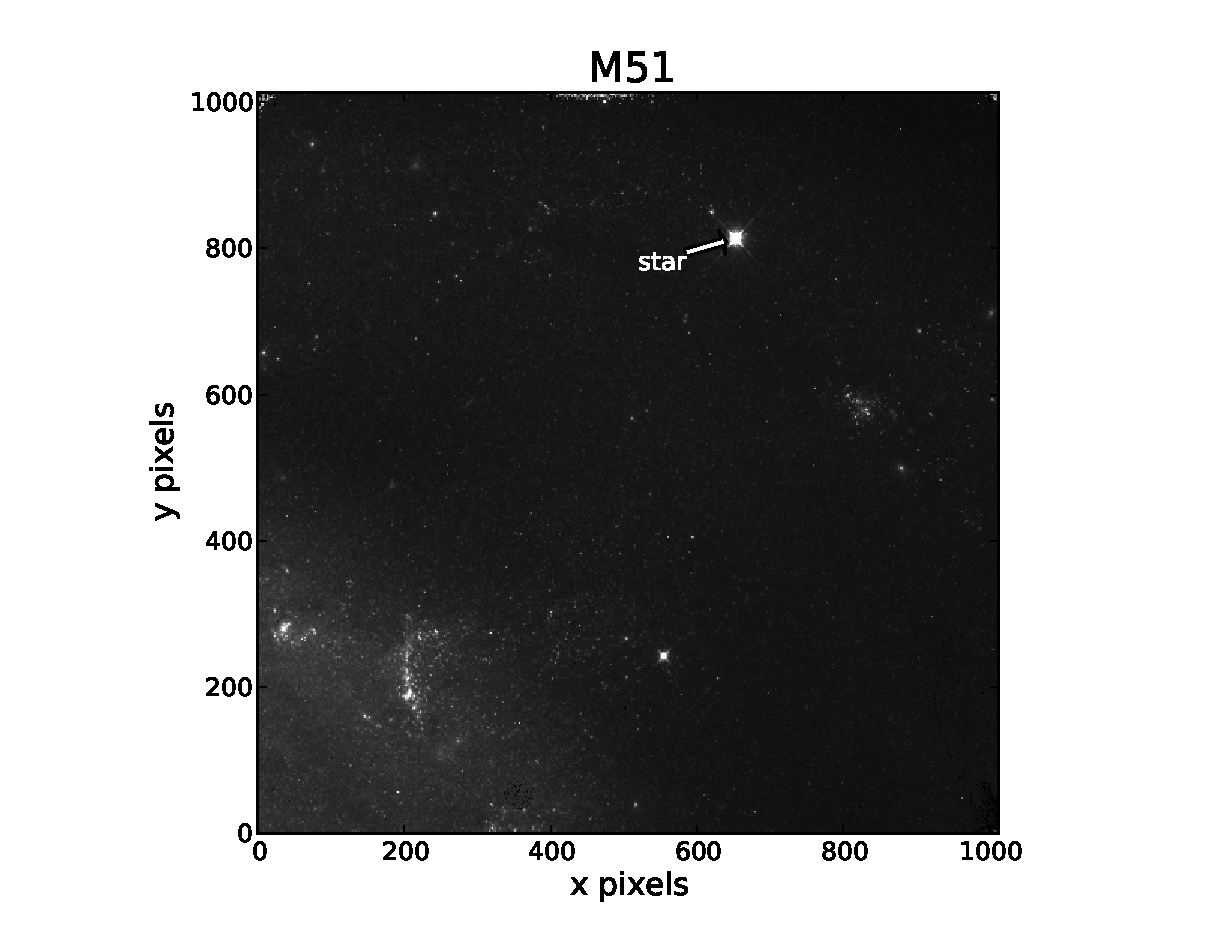
\includegraphics[scale=0.70]{M51.pdf}
    \caption{A corner of the galaxy M51, displayed in greyscale using \textit{pyplot.imshow()}.}
  \label{fig:M51}
\end{figure}
%%%%%%%%%%%%%%%%

For more
plotting options with Matplotlib and PyPlot, check out the 
\href{http://matplotlib.org/}{matplotlib.org} link listed in
Chapter~\ref{ch:links}.  Notice that there is a link to NumPy on this
page, as well as links to screen-shots, thumbnails, and examples.


{\color{blue} {\sf\small EXERCISES}} \\
{\it Exercise \arabic{exercise} \stepcounter{exercise}:  \\
Try plotting a 450$\times$450 pixel cutout of the image (say, the galaxy disk in the lower left corner).
Hint: see Leonardo Ubeda's image plot examples on \href{http://astroplotlib.stsci.edu/}
{http://astroplotlib.stsci.edu/}}


% CONSIDER ADDING:
% Plotting Spectra
% Histograms
% Fitting Lines